\subsection{}
% latex table generated in R 4.2.1 by xtable 1.8-4 package
% Wed Dec  6 21:45:13 2023
\begin{table}[ht]
\centering
\begin{tabular}{llllllr}
  \hline
var & median & mean & min & max & sd & NAs \\ 
  \hline
agro\_emp & 18.6 & 25.1 & 0.1 & 86.3 & 22.3 &  30 \\ 
  bribery & 11.7 & 17.0 & 0.0 & 67.1 & 14.7 &  87 \\ 
  gfce & 16.5 & 17.7 & 5.1 & 62.9 & 8.4 &  36 \\ 
  literacy & 93.0 & 83.6 & 24.2 & 100.0 & 19.3 &  61 \\ 
  log\_gdp & 9.4 & 9.3 & 6.6 & 11.6 & 1.2 &  22 \\ 
  pop\_total & 6.2e+06 & 3.4e+07 & 1.1e+04 & 1.4e+09 & 1.4e+08 &   2 \\ 
  self\_emp & 35.0 & 40.9 & 0.4 & 94.8 & 27.0 &  30 \\ 
  stocks & 6.4 & 28.8 & 0.0 & 538.7 & 66.8 & 131 \\ 
  sample\_size & 715.1 & 3.6e+03 & 120.1 & 1.4e+05 & 1.3e+04 &   2 \\ 
   \hline
\end{tabular}
\caption{Descriptive statistics} 
\label{desc}
\end{table}



\subsection{}
\subsubsection*{(a)}


\begin{figure}[htbp]
  \centering
  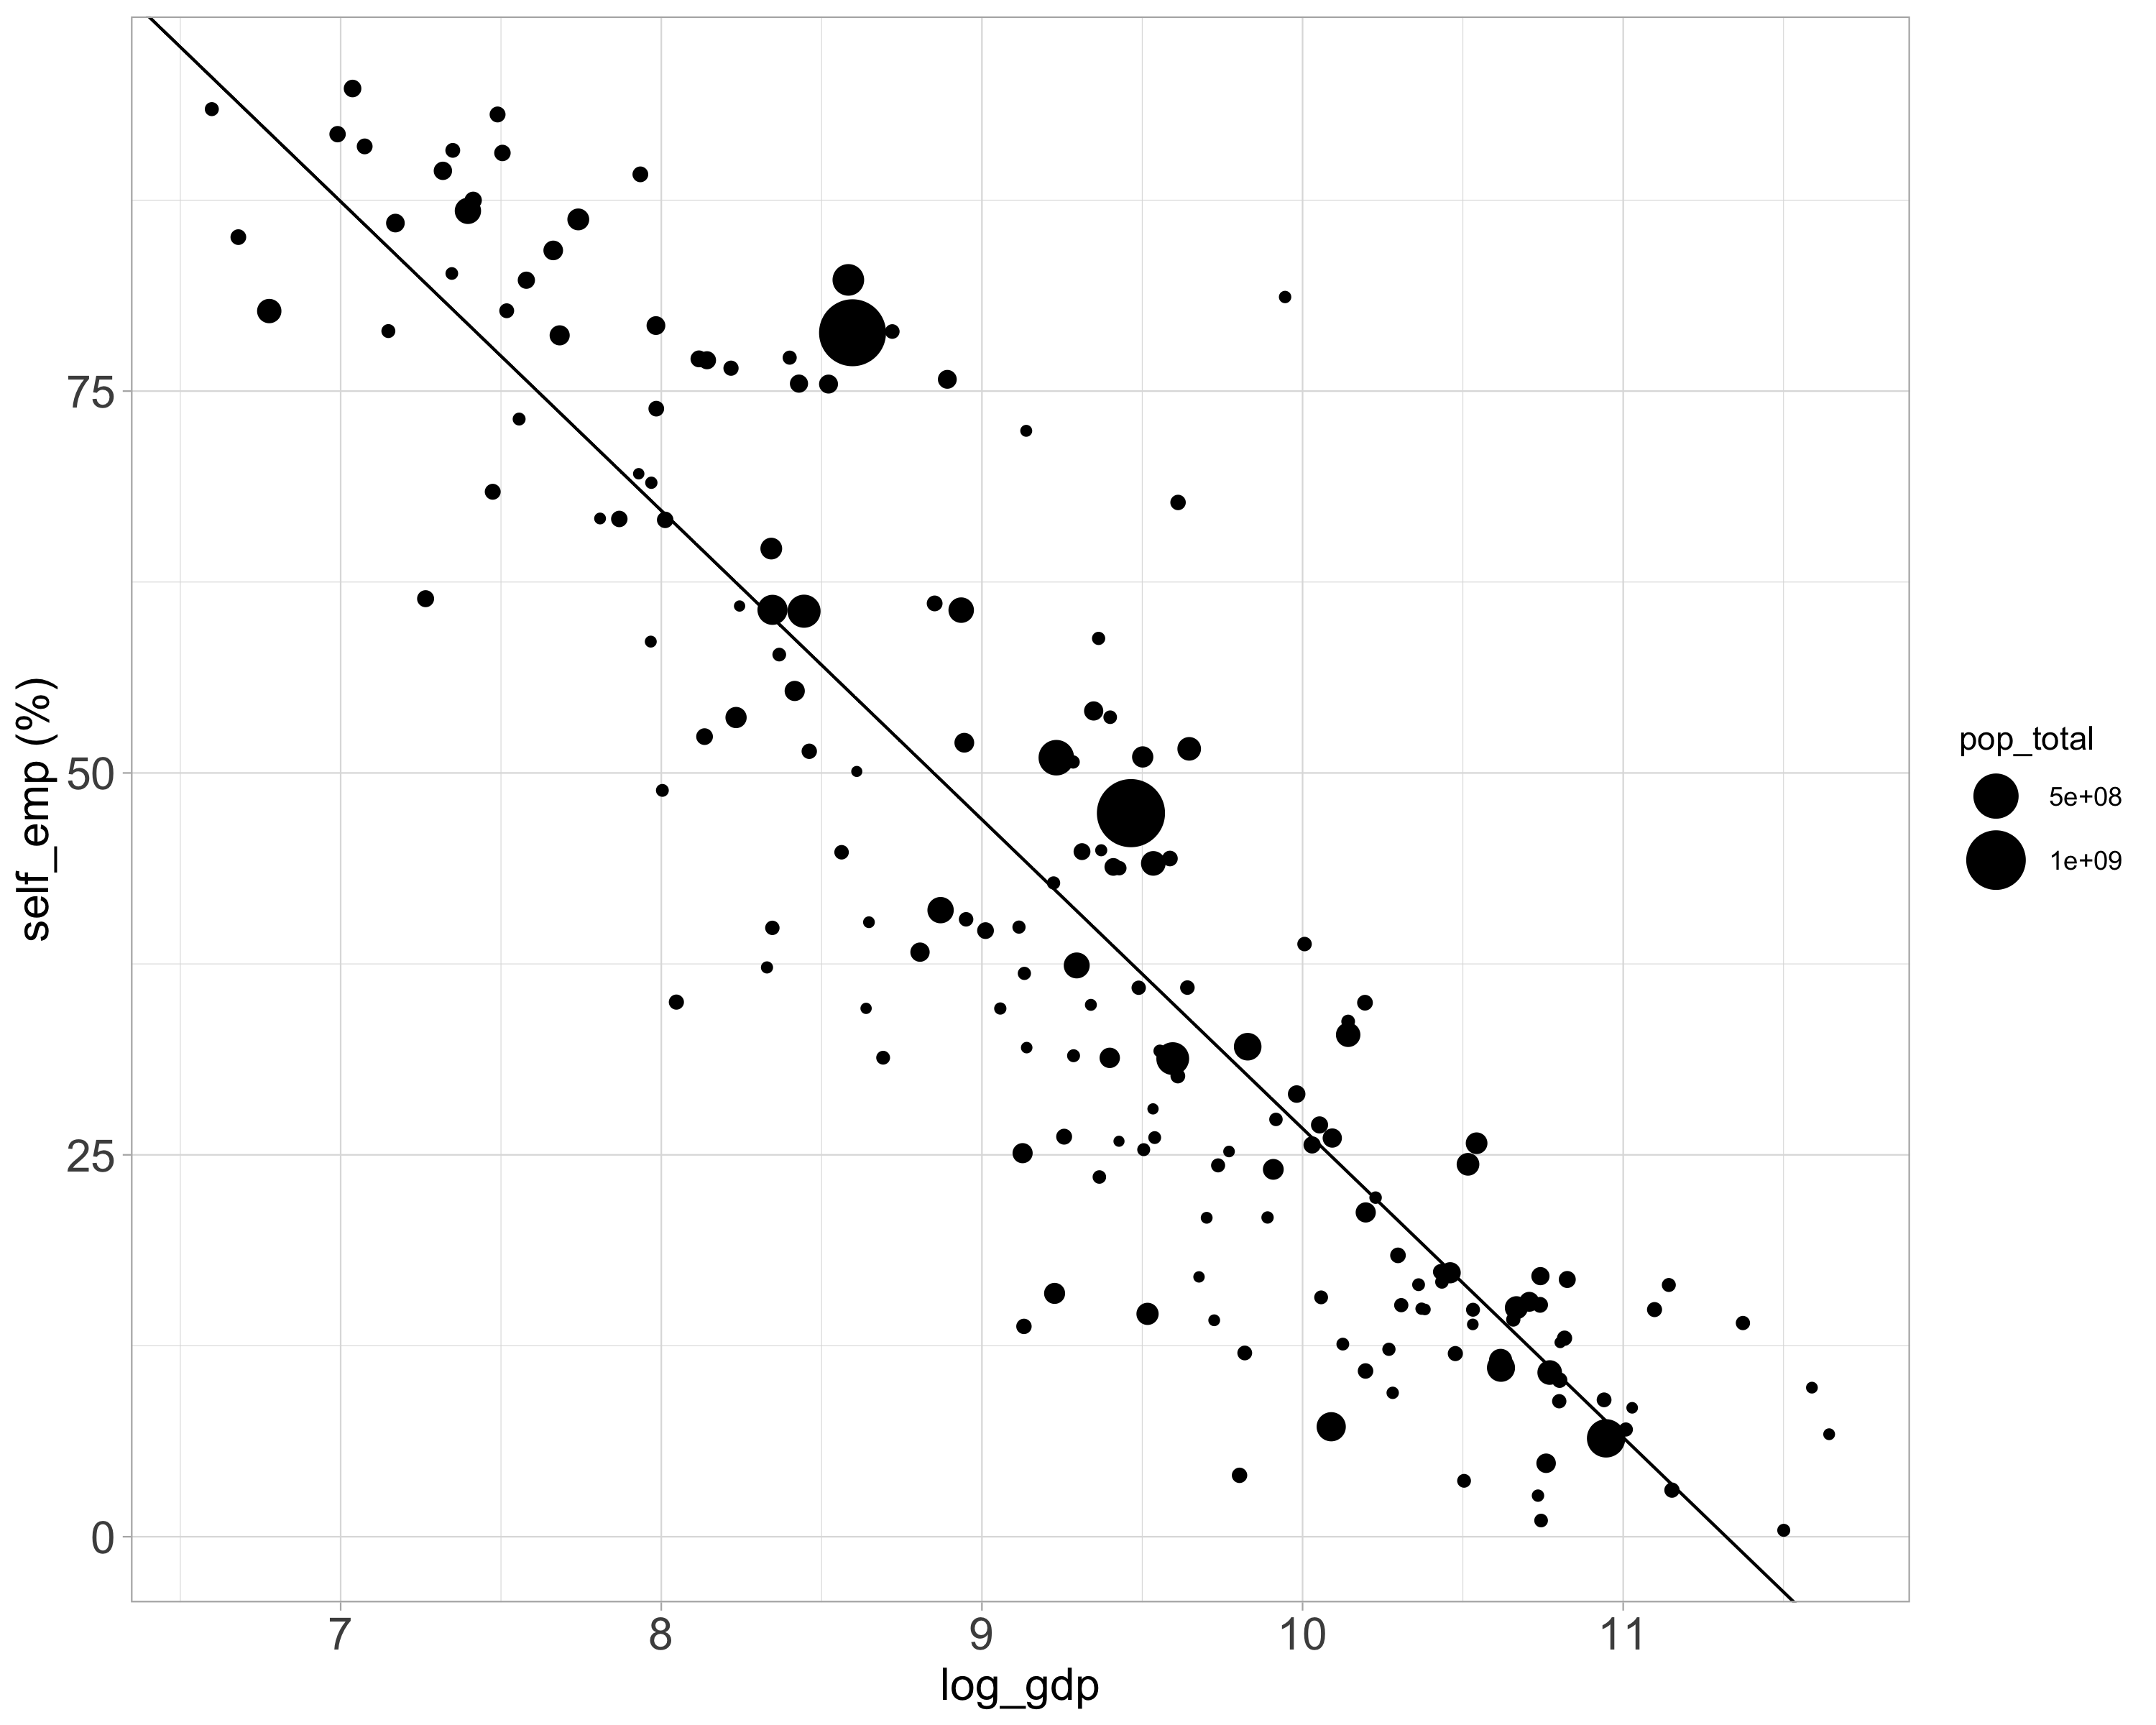
\includegraphics[width=0.8\textwidth]{Exercise_1/OUTPUT/emp_wrt_gdp.png}
  \caption{Self employment rate with respect to GDP}
  \label{fig:emp_gdp}
\end{figure}


Figure \ref{fig:emp_gdp} shows a clear negative relationship between the share of self employment and gdp. The empirical correlation coefficient is equal to $-0.89$
which is very close to $-1$. The anticorrelation is very strong.
\subsubsection*{(b)}

\begin{figure}[htbp]
  \centering
  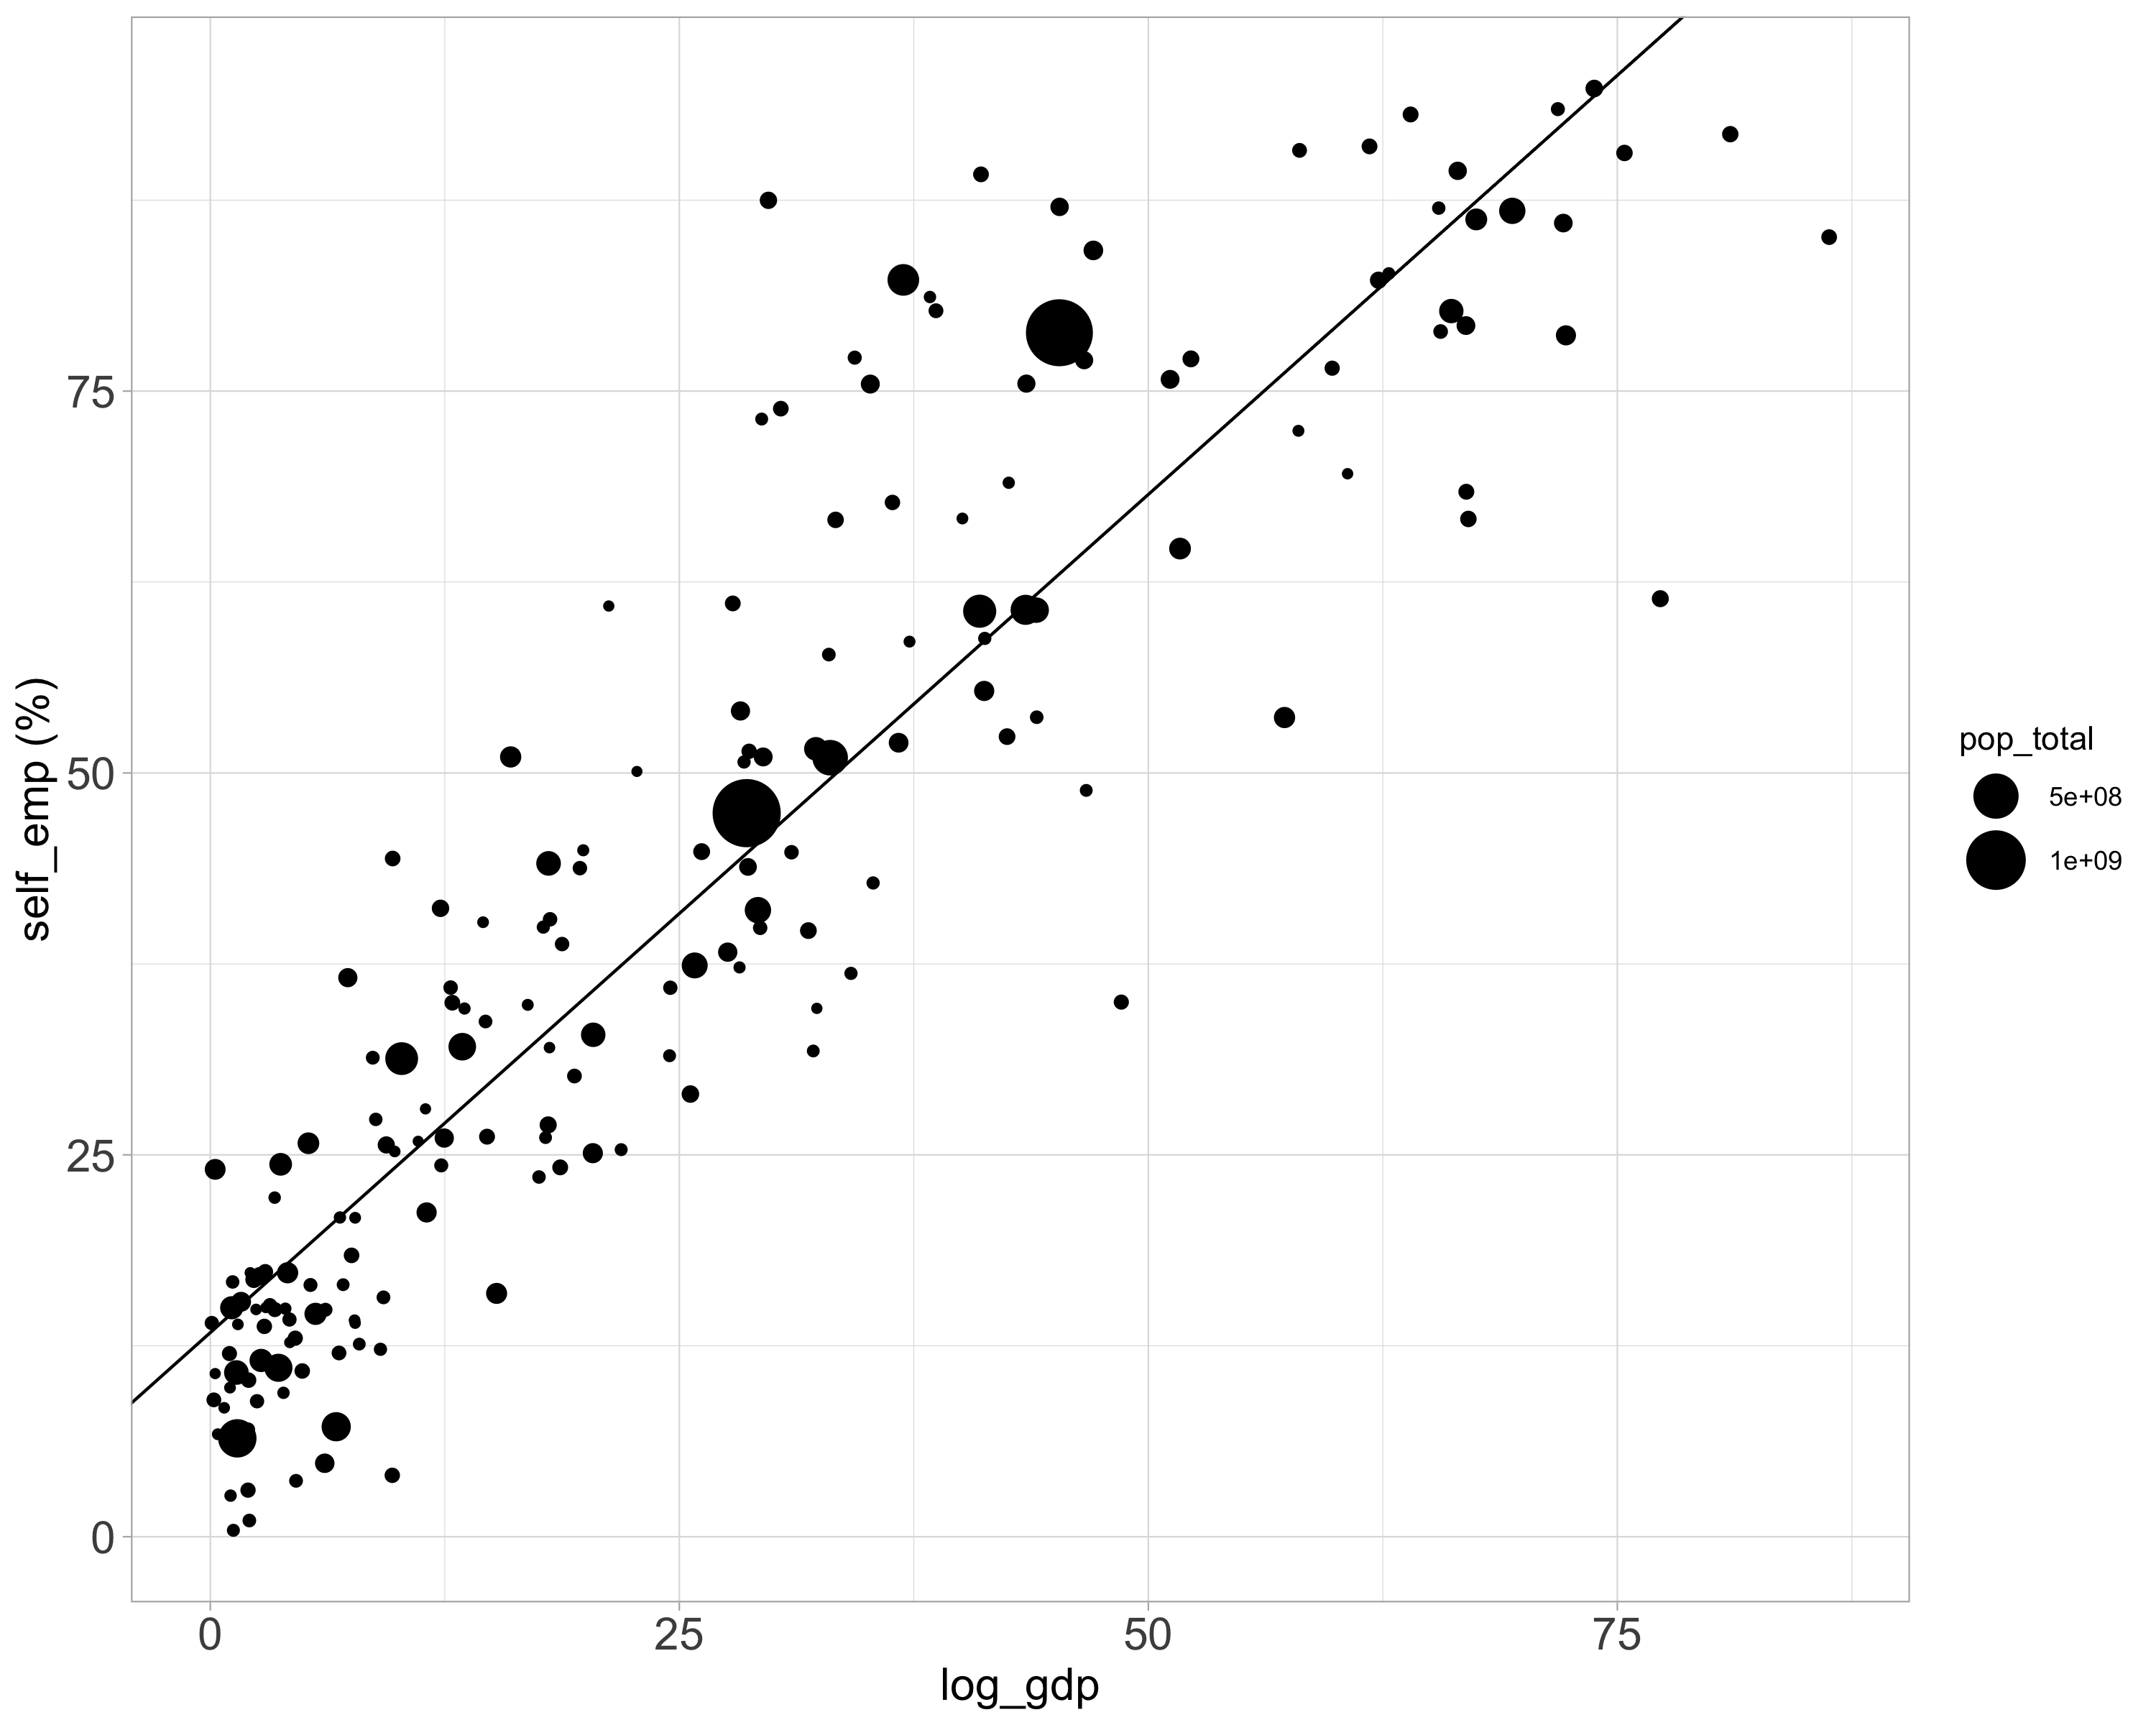
\includegraphics[width=0.8\textwidth]{Exercise_1/OUTPUT/emp_wrt_agro.png}
  \caption{Self employment rate with respect to employment share in the agricultural sector}
  \label{fig:emp_agro}
\end{figure}

As in the previous question, Figure \ref{fig:emp_agro} shows a clear positive relationship between the share of self employment and share of employment in the agricultural sector. The empirical correlation coefficient is equal to $0.91$
which is very close to $1$. The correlation is very strong.

\subsubsection*{(c)}
\begin{figure}[htbp]
  \centering
  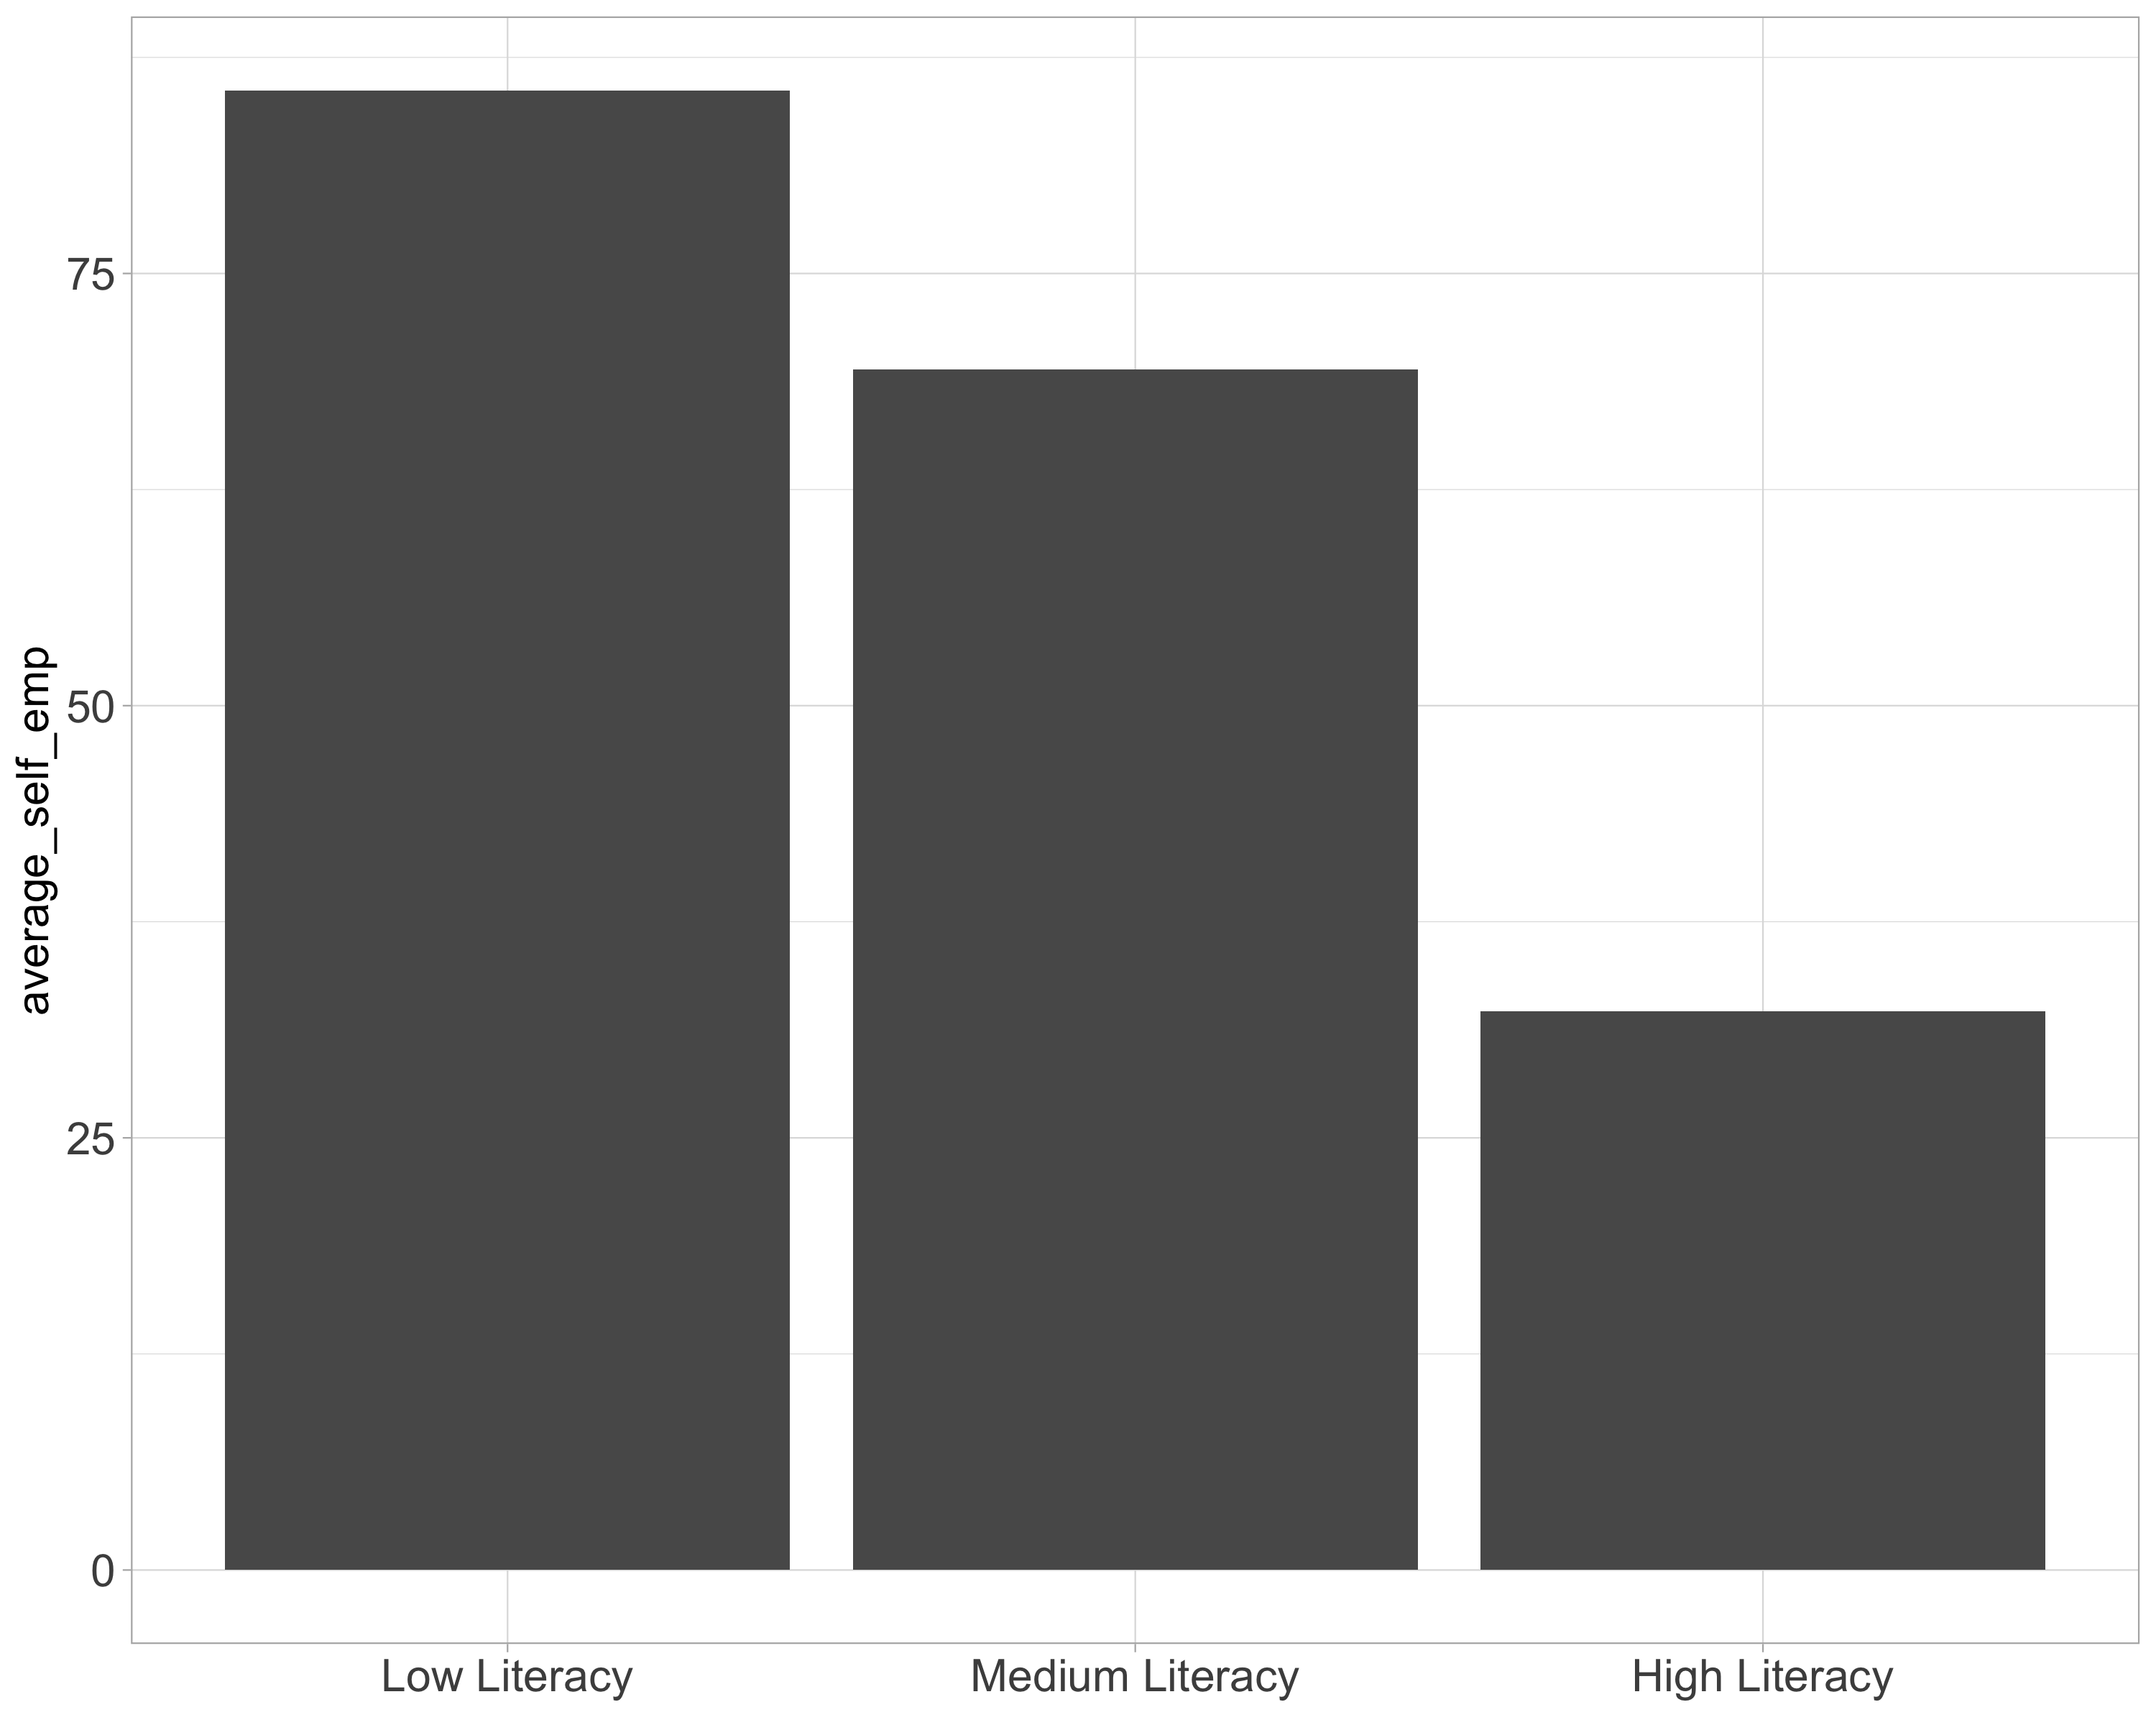
\includegraphics[width=0.8\textwidth]{Exercise_1/OUTPUT/bar_emp_literacy.png}
  \caption{Average self employement rate as a function of the literacy category}
  \label{fig:emp_lit}
\end{figure}

Figure \ref{fig:emp_lit} seems to demonstrate a negative relationship between the literacy category of the population and the self employment rate.

\subsection{}

% Table created by stargazer v.5.2.3 by Marek Hlavac, Social Policy Institute. E-mail: marek.hlavac at gmail.com
% Date and time: Jeu, déc 07, 2023 - 11:24:15
% Requires LaTeX packages: dcolumn 
\begin{table}[!htbp] \centering 
  \caption{Linear Regressions - Exercise 1} 
  \label{results_1} 
\begin{tabular}{@{\extracolsep{5pt}}lD{.}{.}{-3} D{.}{.}{-3} } 
\\[-1.8ex]\hline 
\hline \\[-1.8ex] 
 & \multicolumn{2}{c}{\textit{Dependent variable:}} \\ 
\cline{2-3} 
\\[-1.8ex] & \multicolumn{2}{c}{self\_emp} \\ 
\\[-1.8ex] & \multicolumn{1}{c}{(1)} & \multicolumn{1}{c}{(2)}\\ 
\hline \\[-1.8ex] 
 log\_gdp & -6.506^{***} & -5.520 \\ 
  & (1.755) & (4.042) \\ 
  & & \\ 
 literacy & -0.313^{***} & -0.358^{**} \\ 
  & (0.070) & (0.175) \\ 
  & & \\ 
 agro\_emp & 0.592^{***} & 0.628^{***} \\ 
  & (0.080) & (0.176) \\ 
  & & \\ 
 gfce &  & -0.922^{**} \\ 
  &  & (0.380) \\ 
  & & \\ 
 stocks &  & 0.110^{*} \\ 
  &  & (0.061) \\ 
  & & \\ 
 bribery &  & -0.111 \\ 
  &  & (0.156) \\ 
  & & \\ 
 Constant & 113.219^{***} & 121.953^{***} \\ 
  & (16.361) & (41.265) \\ 
  & & \\ 
\hline \\[-1.8ex] 
Observations & \multicolumn{1}{c}{143} & \multicolumn{1}{c}{49} \\ 
R$^{2}$ & \multicolumn{1}{c}{0.845} & \multicolumn{1}{c}{0.828} \\ 
Adjusted R$^{2}$ & \multicolumn{1}{c}{0.841} & \multicolumn{1}{c}{0.804} \\ 
Residual Std. Error & \multicolumn{1}{c}{10.574 (df = 139)} & \multicolumn{1}{c}{9.262 (df = 42)} \\ 
F Statistic & \multicolumn{1}{c}{252.152$^{***}$ (df = 3; 139)} & \multicolumn{1}{c}{33.720$^{***}$ (df = 6; 42)} \\ 
\hline 
\hline \\[-1.8ex] 
\textit{Note:}  & \multicolumn{2}{r}{$^{*}$p$<$0.1; $^{**}$p$<$0.05; $^{***}$p$<$0.01} \\ 
\end{tabular} 
\end{table} 
